%%% Preamble
\documentclass[paper=letter, fontsize=11pt]{scrartcl}
\usepackage[T1]{fontenc}
\usepackage{fourier}

\usepackage[english]{babel}															% English language/hyphenation
\usepackage[protrusion=true,expansion=true]{microtype}	
\usepackage{amsmath,amsfonts,amsthm} % Math packages
\usepackage[pdftex]{graphicx}	
\usepackage{url}
\usepackage{courier}
\usepackage{listings}
\usepackage[colorlinks = true,
            linkcolor = blue,
            urlcolor  = blue,
            citecolor = blue,
            anchorcolor = blue]{hyperref}

%%% Custom sectioning
\usepackage{sectsty}
\allsectionsfont{\centering \normalfont\scshape}

%%% Custom headers/footers (fancyhdr package)
\usepackage{fancyhdr}
\pagestyle{fancyplain}

\fancyhead{}											% No page header
\fancyfoot[L]{}											% Empty 
\fancyfoot[C]{}											% Empty
\fancyfoot[R]{\thepage}									% Pagenumbering
\renewcommand{\headrulewidth}{0pt}			% Remove header underlines
\renewcommand{\footrulewidth}{0pt}				% Remove footer underlines
\setlength{\headheight}{13.6pt}


%%% Equation and float numbering
\numberwithin{equation}{section}		% Equationnumbering: section.eq#
\numberwithin{figure}{section}			% Figurenumbering: section.fig#
\numberwithin{table}{section}				% Tablenumbering: section.tab#


%%% Maketitle metadata
\newcommand{\horrule}[1]{\rule{\linewidth}{#1}} 	% Horizontal rule

\title{
		%\vspace{-1in} 	
		\usefont{OT1}{bch}{b}{n}
		\normalfont \normalsize \textsc{Udacity Self Driving Car Engineer Nano Degree Program} \\ [25pt]
		\horrule{0.5pt} \\[0.4cm]
		\huge Project 03: Behavioral Cloning \\
		\horrule{2pt} \\[0.5cm]
}
\author{
		\normalfont 								\normalsize
        Thomas Antony\\[-3pt]		\normalsize
        \today
}
\date{}

\usepackage{filecontents}
\begin{filecontents}{\jobname.bib}
@article{nvidia:endtoend2016,
  title={{End to End Learning for Self-Driving Cars}},
  author={{Bojarski, Mariusz and Del Testa, Davide and Dworakowski, Daniel and Firner, Bernhard and Flepp, Beat and Goyal, Prasoon and Jackel, Lawrence D and Monfort, Mathew and Muller, Urs and Zhang, Jiakai and others}},
  journal={{arXiv preprint arXiv:1604.07316}},
  year={2016}
}
\end{filecontents}

%%% Begin document
\begin{document}
\maketitle
\section{Running the Model}
The Keras model is stored in the file \emph{model\_5.json} with the weights being stored in \emph{model\_5.h5}. Run the model using the command:

\begin{lstlisting}[language=bash]
$ python drive.py model_5.json
\end{lstlisting}

\texttt{}

\emph{drive.py} pre-processes the telemetry obtained from the simulator and passes it along to the Keras model for predicting the steering angle. It also has a rudimentary "cruise-control" system for setting the throttle to achieve a target speed. It was found that the model is able to drive on Track 1 at 30 mph and navigate Track 2 at speeds of up to 20 mph.

In order to obtain the live trainer code, be sure to run the following command after cloning the repository.

\begin{lstlisting}[language=bash]
$ git submodule update --init --recursive --remote
\end{lstlisting}

\section{Model Architecture and Training Strategy}

\subsection{Neural Network Architecture}
Multiple training architectures based on Convolutional Neural Networks were evaluated. Most of them failed. Transfer learning with VGG16 and Inception v3 was also attempted. Finally, the architecture described in NVIDIA's End-To-End deep learning paper\cite{nvidia:endtoend2016} was used. This architecture was chosen at the end after experimenting with many others, primarily due to the small size and hence low processing latency. A normalization layer was added on top of the network to normalize the input images.

The use of the live training methodology described in Section~\ref{sec:live_training} also helped getting this model to work. Additional models were not tested using the live training strategy due to lack of time. The model architecture is shown in Fig.~\ref{fig:model_arch}.

\begin{figure}[!htbp]
  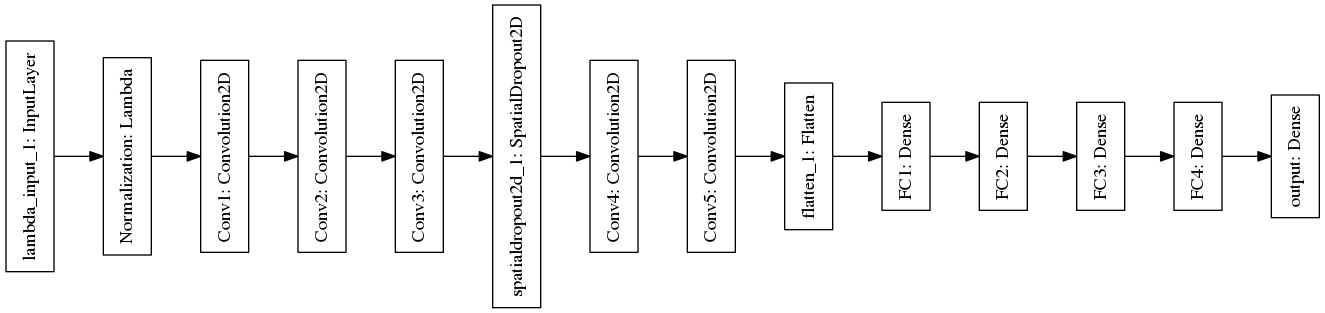
\includegraphics[width=\linewidth]{model.png}
  \caption{Model architecture}
  \label{fig:model_arch}
\end{figure}

The architecture does not contain any dropout layers. The MSE of the model was always above 0.01 for working versions and so there doesn't seem to be much overfitting going on. However, to be sure of this, a model can be trained on just data from track 1 and tested on track 2. This wasn't done due to time constraints as the focus was on getting at least one model that worked on one or both tracks. To further test for "memorizing" the track, the car was also tested by deliberately perturbing it's path from time to time and it was found that it always returned to the center of the lane.

During the initial training step, a separate dataset was generated and used for testing. A validation dataset with 10\% of the original dataset was also used. Further more, live testing + training was also performed as described in the upcoming sections. The resulting model is able to drive on track 1 at 30 mph and track 2 at 20 mph.

\subsection{Training Strategies}

Two separate strategies were used for training the model. The first was a batched training strategy using data collected from the "Training mode" of the simulator. This is done is \emph{train\_model.ipynb}. The model was then further fine tuned with a low learning rate using a live trainer that was developed specifically for this purpose. This is further discussed in Section~\ref{sec:live_training}

\subsubsection{Batched training}
\label{sec:batched_training}

The Jupyter Notebook \emph{train\_model.ipynb} contains the code used to train the model initially. The dataset obtained from the simulator consisted of image files and a CSV file. The CSV file was loaded into a pandas dataframe and randomized. Data was collected for both straight lane-keeping and recovery from perturbations. Both tracks were driven in both directions and data was collected. 

An image generator that takes the pandas dataframe as input and generates batches of training data was developed. This can be seen in the \texttt{batch\_generator} method in the notebook. The generator can run indefinitely and starts over the from the beginning when it runs out of data. The data set was augmented by also using the right and left camera images with a 1.5 degree shift to the original steering angle. This resulted in a total of around 24000 images (starting from 8000 original data points). The input images were converted to YUV color space and a $240\times80$ region of the image was cropped out. This region starts under the horizon, removes most of the exterior environment and focuses on the road. This is similar to what was done in the NVIDIA paper \cite{nvidia:endtoend2016}. The image was then resized to $200\times66$ before being passed into the model.

The ADAM optimizer with a learning rate of $0.0001$ was used. The data was trained over 6 epochs of 24000 samples each.

\subsubsection{Live training}
\label{sec:live_training}

The live trainer allows manual override of the model while it drives the car in autonomous mode. The car can then be controlled using the keyboard and there is also the option to collect the data being generated at this time and use it to fine-tune the model. More details can be seen in the ReadMe file of the \href{https://github.com/thomasantony/sdc-live-trainer/blob/master/README.md}{live trainer} and this \href{https://medium.com/@tantony/training-a-neural-network-in-real-time-to-control-a-self-driving-car-9ee5654978b7}{article}. The live trainer can also be found as a sub-module in the project repository. 

The live trainer was used to collect additional data in portions of the track where the model was failing to navigate. This was done by considerably slowing down the car when approaching these sections and then driving manually through the area while simultaneously collecting data and training the model. This way, the model was able to learn to get through these spots where the original dataset was probably lacking in data. During the live training, the learning rate was further reduced to $1e-6$ to prevent corruption of existing weights from any sudden mistakes during manual driving. 

\subsection{Cruise Control Implementation}
Th cruise control was implemented as a simple proportional gain controller. The throttle was computed from the speed feedback available in the telemetry.

\[
T = K_p \left(v_{target} - v\right)
\]
where $T$ is the throttle, $K_p$ is the proportional gain and $v_{target}$ and $v$ are the targeted and current speeds respectively. The gain was picked to be 0.35. This was able to get the speed within $\pm 1$ mph of the target speed.

\bibliographystyle{abbrv}
\bibliography{\jobname} 
%%% End document
\end{document}